% This file was generated with po4a. Translate the source file.
%


\documentclass[a4paper]{article}
\usepackage[T1]{fontenc}
\usepackage[usenames,dvipsnames]{xcolor}
\usepackage{tikz}
\usepackage{framed}
\usepackage{multicol}
\usepackage{fontspec}
\pagestyle{plain}   
\usepackage{ragged2e} 
\usepackage{etoolbox}
\AtBeginEnvironment{multicols}{\RaggedRight}
\definecolor{topblue}{RGB}{29, 56,56}
\definecolor{bottombrown}{RGB}{75, 79, 47}

\usepackage{graphicx}
\usepackage[top=0mm, bottom=0mm, left=0mm, right=0mm]{geometry}
\begin{document}

\hspace{-0.55cm}\begin{tikzpicture}

\setmainfont{DejaVu Serif} \fontsize{1.3cm}{0.9cm} 

\selectfont

\fill [topblue] (0mm,0.5\paperheight) rectangle
(\paperwidth+0.05cm,\paperheight);

\fill [bottombrown] (0mm,0mm) rectangle
(\paperwidth+0.05cm,0.5\paperheight);

\node [below, white] at (0.5\paperwidth, \paperheight-5mm)  {ЗАЩИТИ СВОЙ
EMAIL};

\fontsize{0.65cm}{0.75cm} 

\selectfont

\node [below, white, align=center, text width=0.95\paperwidth] at
(0.5\paperwidth, \paperheight-25mm)  {Массовая слежка нарушает наши
важнейшие права и делает выражение мыслей рискованным};

\node [below, white, align=center, text width=0.95\paperwidth, font=\bf] at
(0.5\paperwidth, \paperheight-42mm)  {Но мы далеко не беззащитны и можем
кое-что сделать};

\node [below, inner sep=0,outer sep=0] at (0.5\paperwidth,
\paperheight-60mm) {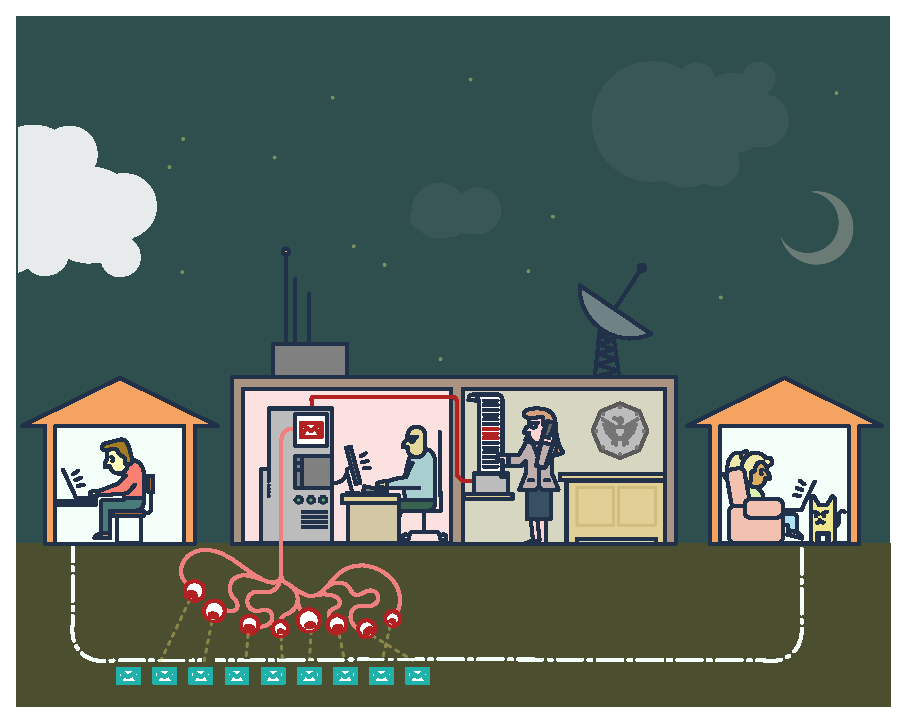
\includegraphics[width=\paperwidth]{leaflet-1_1.eps}};
\fontsize{0.55cm}{0.6cm} \selectfont

\node [below, white, align=center, text width=0.95\paperwidth, font=\bf] at
(0.5\paperwidth, \paperheight-225mm)  { \begin{multicols}{3} Пароль на вашей
почте -- лишь тонкий слой, он не защитит вас от тарана хитроумных систем
слежки. \par \columnbreak Каждое письмо на пути к адресату проходит через
множество компьютеров. Агенства слежки пользуются этим, чтобы читать
миллионы писем.  \par \columnbreak Даже если вам нечего скрывать, когда вы
шлете обычное письмо, те, с кем вы общаетесь, тоже подвергаются
слежке. \end{multicols} };

\end{tikzpicture}




\end{document}
